\documentclass[11pt,a4paper]{article}

% ------------------------------------------------------------------ packages
\usepackage[T1]{fontenc}
\usepackage[utf8]{inputenc}
\usepackage{lmodern}
\usepackage{microtype}
\usepackage[margin=2.4cm]{geometry}
\usepackage{amsmath,amssymb,bm}
\usepackage{booktabs,tabularx,multirow,array}
\usepackage{graphicx}
\usepackage[table]{xcolor}
\usepackage{tikz}
\usetikzlibrary{arrows.meta,positioning,shapes.geometric,fit,backgrounds,calc}
\usepackage{pgfplots}
\pgfplotsset{compat=1.18}
\usepackage{enumitem}
\setlist{itemsep=2pt,topsep=4pt}
\usepackage[authoryear,round]{natbib}
\usepackage{caption}
\captionsetup{font=small,labelfont=bf}
\usepackage{float}
\usepackage[section]{placeins}
\usepackage[hidelinks]{hyperref}
\usepackage[nameinlink,capitalise]{cleveref}

\definecolor{accent}{HTML}{2B5C8A}
\definecolor{warn}{HTML}{B5462E}
\definecolor{ok}{HTML}{2E7D4F}
\definecolor{muted}{HTML}{6B7280}
\definecolor{paneA}{HTML}{EAF1F8}
\definecolor{paneB}{HTML}{FDF1E7}
\definecolor{paneC}{HTML}{EDF7F0}

\newcommand{\code}[1]{\texttt{\small #1}}
\newcommand{\sev}[1]{\textbf{\textcolor{warn}{#1}}}
\newcommand{\Dt}{\tilde D}
\newcommand{\Gt}{\tilde G}

\title{\textbf{MatchSense AI}: A News-Aware, Lineup-Conditioned Forecasting
System for the English Premier League\\[4pt]
\large Architecture, Walk-Forward Evaluation, and a Critical Appraisal}
\author{Shaurya Jain\thanks{Independent technical report, November 2026.
All numerical results are produced by the repository's own scripts and
artifacts (Appendix~\ref{app:repro}).}}
\date{4 November 2026}

\begin{document}
\maketitle

% ------------------------------------------------------------------ abstract
\begin{abstract}
\noindent
MatchSense AI answers natural-language questions such as \emph{``Will
Manchester City win tonight?''}. It resolves the question to a verified fixture
in the user's timezone and gathers 72 hours of news for both clubs. It turns
that text into typed, sourced availability evidence, predicts both starting
line-ups probabilistically, and adjusts a pre-existing recency-weighted Poisson
score model through a separately estimated line-up layer, combined by Monte
Carlo simulation. Its central design rule is that the language model
\emph{never} produces a probability. It only reads text, and every number comes
from a fitted statistical model whose out-of-sample behaviour has been measured.
We evaluate each component with leakage-controlled, chronological protocols.
The baseline goal model beats a class-frequency prior on an untouched season
(log loss $1.028$ vs.\ $1.082$), and a multinomial-logistic alternative adds
nothing (selected blend weight $0\%$). A pooled logistic start-probability model
is clearly useful (test log loss $0.400$ vs.\ $0.461$; top-11 precision $0.798$
vs.\ $0.742$). However, \emph{line-up effects on goal rates could not be
identified} from the one season of line-up data available. Player-level ridge
effects that won on validation lost on test (up to $+0.027$ log loss, 95\% CI
$[+0.000,+0.053]$), and no team-level specification improved held-out log loss
with an interval excluding zero. The deployed line-up layer is therefore an
explicitly labelled, prior-dominated Bayesian model, and the unadjusted baseline
is always shown beside it. We document three evaluation rounds, each changed
after viewing test results, and conclude that the test folds are no longer a
clean holdout. We then give a systematic appraisal of the system's strengths,
flaws and threats to validity, including model artefacts found by replaying the
system. Examples are that a goalkeeper's absence is attributed mainly to his own
team's attack, and that a draw is never the most likely outcome.
\end{abstract}
\newpage

\noindent\textbf{Keywords:} football forecasting; Poisson regression;
Dixon--Coles; line-up prediction; information extraction; large language
models; Monte Carlo simulation; data leakage; proper scoring rules; negative
results.

\tableofcontents
\newpage

% ================================================================== 1
\section{Introduction}\label{sec:intro}

Statistical models of football results have a long history. It runs from
independent Poisson goal models \citep{maher1982} and the low-score dependence
correction of \citet{dixon1997}, through rating systems such as Elo
\citep{elo1978,hvattum2010}, to bivariate, Bayesian-hierarchical and dynamic
formulations \citep{karlis2003,rue2000,baio2010,koopman2015} and machine-learned
feature models \citep{hubacek2019,bunker2019}. These models are built from
results and schedules. Much of the information that practitioners consider
decisive before a match is not in a results table. It arrives as unstructured
text: injury bulletins, suspensions, press-conference remarks, predicted and
confirmed line-ups.

Large language models (LLMs) make such text easy to read and equally easy to
misuse. An LLM asked ``will City win?'' produces a fluent answer with no
calibrated probabilistic meaning and a well-documented tendency to hallucinate
\citep{ji2023}. Retrieval augmentation \citep{lewis2020} grounds the text the
LLM sees, but it does not make the model's numerical claims calibrated.
MatchSense is built around the opposite division of labour:

\begin{quote}
\emph{The LLM is an information-extraction and query-understanding component
whose output schemas contain no probability fields. All probabilities come from
fitted statistical models, and when the measured evidence for a component is
weak, the system says so in every response.}
\end{quote}

\paragraph{Contributions.}
\begin{enumerate}
  \item \textbf{An architecture} (\cref{sec:system}) that layers news- and
        line-up-derived adjustments on top of an \emph{unchanged}, independently
        validated baseline through an offset Poisson GLM, so the baseline always
        remains available for comparison.
  \item \textbf{A leakage-controlled evaluation} (\cref{sec:design,sec:results})
        of the baseline, the selection model and twenty-two line-up-impact
        candidates, with matchday walk-forward folds and paired bootstrap
        intervals.
  \item \textbf{A negative result, reported with its history}
        (\cref{sec:rounds}). Line-up effects on goal rates are not identifiable
        from one season, and the most expressive models overfit. We disclose
        three post-hoc evaluation rounds.
  \item \textbf{A critical appraisal} (\cref{sec:appraisal}): strengths,
        concrete flaws with severity ratings, a pros/cons comparison against
        simpler alternatives, threats to validity, and responsible-use
        considerations.
\end{enumerate}

% ================================================================== 2
\section{Related work}\label{sec:related}

\paragraph{Goal-based models.}
\citet{maher1982} modelled home and away goals as independent Poisson variables
with attack and defence parameters. \citet{dixon1997} added a dependence
correction $\tau_\rho$ for scores of 0--0, 1--0, 0--1 and 1--1, and
exponential time-weighting of past matches. Both ideas appear in our baseline
as recency weights and a Dixon--Coles score grid. \citet{karlis2003} introduced
bivariate Poisson models. \citet{rue2000} and \citet{koopman2015} let team
strengths evolve over time, and \citet{baio2010} placed the parameters in a
Bayesian hierarchy, which shrinks weakly identified effects. That last idea is
central to our handling of line-up effects.

\paragraph{Ratings and feature models.}
Elo ratings \citep{elo1978} are competitive predictors of football outcomes
\citep{hvattum2010} and serve as inputs to our baseline. Feature-based
learners, from gradient-boosted trees on relational features
\citep{hubacek2019} to generic ML pipelines \citep{bunker2019}, typically gain
little over well-specified goal models once proper scoring rules are used.
Our walk-forward comparison of Poisson and multinomial-logistic models agrees
(\cref{sec:res-baseline}).

\paragraph{Player contribution.}
Regularised adjusted plus-minus estimates individual contributions by ridge
regression \citep{hoerl1970} on line-up indicators \citep{sill2010}.
\citet{kharrat2020} adapted plus-minus to football and stressed heavy
regularisation and multi-season data. Action-value models such as VAEP
\citep{decroos2019} use event streams that are not available to us. Our failure
to identify player effects from one season is consistent with these
observations.

\paragraph{Forecast evaluation and leakage.}
We use strictly proper scoring rules \citep{gneiting2007}: logarithmic loss,
the Brier score \citep{brier1950} and the ranked probability score
\citep{epstein1969}, which \citet{constantinou2012} recommend for ordered
football outcomes. Evaluation is rolling-origin \citep{tashman2000}.
Temperature scaling follows \citet{guo2017}. Selection-induced optimism when
the same data guide model choice and performance estimation is analysed by
\citet{cawley2010}, and the one-standard-error rule by \citet{hastie2009}.
Leakage is formalised by \citet{kaufman2012}.

\paragraph{Sampling and uncertainty.}
Line-ups are sampled with the Gumbel-top-$k$ trick \citep{kool2019}, an
approximation to conditional Bernoulli sampling \citep{chen1994}. Coefficient
uncertainty uses a Laplace approximation \citep{tierney1986}. Paired intervals
use the bootstrap \citep{efron1993}. Near-duplicate news detection uses word
shingles \citep{broder1997}.

% ================================================================== 3
\section{System overview}\label{sec:system}

\Cref{fig:arch} shows the request path. The system is a Python package
(\code{src/matchsense/}, about 4{,}500 lines) served by FastAPI with a
build-free JavaScript dashboard. It runs in two modes. \emph{Live} mode uses
public endpoints and optional API keys. \emph{Demo} mode replays a recorded
snapshot of the Fantasy Premier League (FPL) endpoints with \emph{simulated}
news, which is clearly labelled as such.

\begin{figure}[t]
\centering
\resizebox{\linewidth}{!}{%
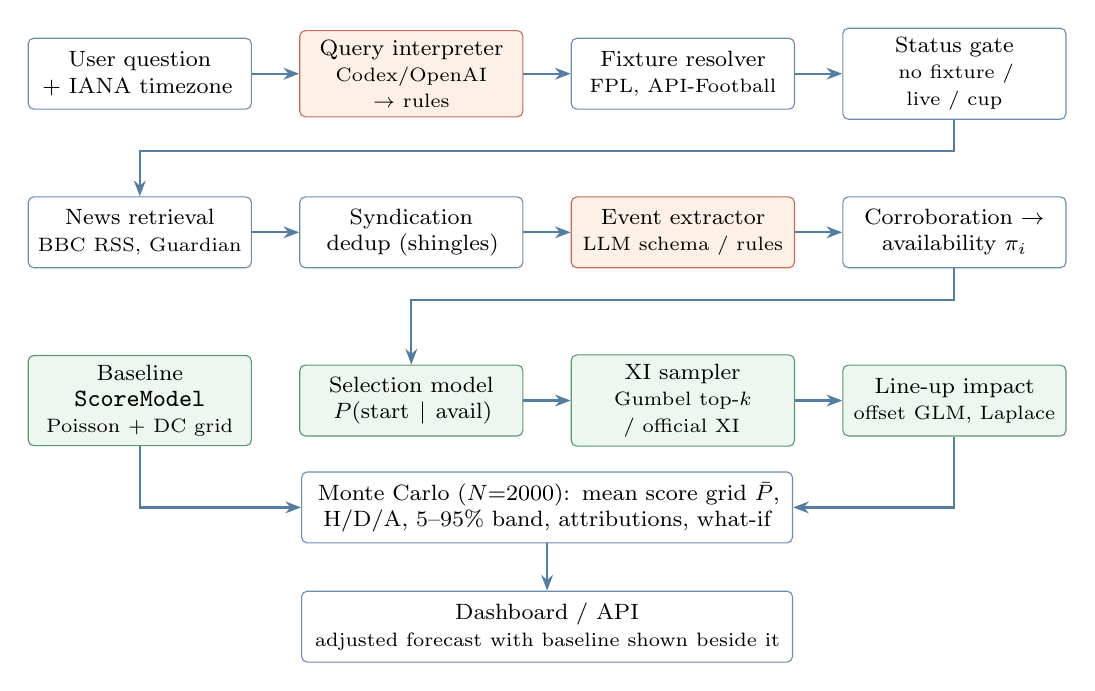
\begin{tikzpicture}[
  node distance=5mm and 6mm,
  box/.style={draw=accent!70,rounded corners=2pt,fill=white,align=center,
              font=\footnotesize,minimum height=9mm,text width=26mm},
  llm/.style={box,draw=warn!80,fill=paneB},
  stat/.style={box,draw=ok!80,fill=paneC},
  arr/.style={-{Stealth[length=2mm]},thick,accent!80}]
  \node[box] (q) {User question\\+ IANA timezone};
  \node[llm,right=of q] (interp) {Query interpreter\\{\scriptsize Codex/OpenAI $\to$ rules}};
  \node[box,right=of interp] (fix) {Fixture resolver\\{\scriptsize FPL, API-Football}};
  \node[box,right=of fix] (status) {Status gate\\{\scriptsize no fixture / live / cup}};

  \node[box,below=11mm of q] (news) {News retrieval\\{\scriptsize BBC RSS, Guardian}};
  \node[box,right=of news] (dedup) {Syndication\\dedup (shingles)};
  \node[llm,right=of dedup] (extract) {Event extractor\\{\scriptsize LLM schema / rules}};
  \node[box,right=of extract] (avail) {Corroboration $\to$\\availability $\pi_i$};

  \node[stat,below=11mm of news] (base) {Baseline\\\code{ScoreModel}\\{\scriptsize Poisson + DC grid}};
  \node[stat,right=of base] (sel) {Selection model\\$P(\text{start}\mid\text{avail})$};
  \node[stat,right=of sel] (xi) {XI sampler\\{\scriptsize Gumbel top-$k$ / official XI}};
  \node[stat,right=of xi] (imp) {Line-up impact\\{\scriptsize offset GLM, Laplace}};

  \node[box,below=9mm of $(sel)!0.5!(xi)$,text width=60mm] (mc) {Monte Carlo ($N{=}2000$): mean score grid $\bar P$,\\
        H/D/A, 5--95\% band, attributions, what-if};
  \node[box,below=6mm of mc,text width=60mm] (ui) {Dashboard / API\\{\scriptsize adjusted forecast with baseline shown beside it}};

  \draw[arr] (q) -- (interp);
  \draw[arr] (interp) -- (fix);
  \draw[arr] (fix) -- (status);
  \draw[arr] (status.south) |- ++(0,-4mm) -| (news.north);
  \draw[arr] (news) -- (dedup);
  \draw[arr] (dedup) -- (extract);
  \draw[arr] (extract) -- (avail);
  \draw[arr] (avail.south) |- ++(0,-4mm) -| (sel.north);
  \draw[arr] (sel) -- (xi);
  \draw[arr] (xi) -- (imp);
  \draw[arr] (base.south) |- (mc.west);
  \draw[arr] (imp.south) |- (mc.east);
  \draw[arr] (mc) -- (ui);
\end{tikzpicture}}
\caption{Request path. Orange boxes use an LLM, but only to emit
\emph{structure} (intent, clubs, date phrase, typed events). Green boxes are
fitted statistical components that produce all numbers. Each LLM stage has a
deterministic fallback.}
\label{fig:arch}
\end{figure}

\Cref{tab:modules} maps the components to source files.

\begin{table}[h]
\centering\small
\begin{tabularx}{\linewidth}{@{}lX@{}}
\toprule
Module & Responsibility \\
\midrule
\code{interpreter.py} & LLM query understanding (Codex CLI $\to$ OpenAI API $\to$ rule parser); strict JSON schema; validated and cached per question. \\
\code{query.py}, \code{teams.py} & Club aliases, intent, timezone-aware windows (``tonight'' = 17:00--06:00 local), what-if player phrases. \\
\code{providers/} & FPL, openfootball, API-Football, football-data.org, BBC/Guardian/NewsAPI/GNews; demo replay. \\
\code{http.py} & SQLite response cache, retries with back-off, per-host throttling, stale fallback. \\
\code{intelligence.py} & Syndication clustering, LLM/rule extraction (Pydantic), corroboration into availability beliefs. \\
\code{players.py} & Name-to-squad identity resolution (initials, accents, particles; refuses ambiguous matches). \\
\code{lineup\_data.py}, \code{training.py} & Leakage-safe selection state; walk-forward folds; one-SE rule; bootstrap. \\
\code{impact.py}, \code{lineups.py} & Offset-Poisson line-up GLM (MAP + Laplace); selection model; constrained XI sampling. \\
\code{baseline.py}, \code{simulate.py} & Existing \code{ScoreModel} + season roll-forward; Monte Carlo score grids. \\
\code{pipeline.py}, \code{storage.py}, \code{api.py} & Orchestration, explanations, what-if, prediction history and scoring, HTTP API. \\
\bottomrule
\end{tabularx}
\caption{Principal modules.}
\label{tab:modules}
\end{table}

% ================================================================== 4
\section{Data}\label{sec:data}

\paragraph{Historical results.}
9{,}880 completed Premier League matches (2000-01 to 2025-26) from
the \code{openfootball/}\allowbreak\code{england} repository \citep{openfootball}, ingested into a normalised
PostgreSQL schema by the project's existing pipeline. The pipeline uses
explicit team aliases, rejects duplicate and impossible scores, and stores a
fingerprint and the raw source text for each match.

\paragraph{Historical line-ups.}
Only 2025-26 has full line-up files locally: 380 matches with eleven parsed
starters per side, substitution minutes and scorers. This single season is the
\emph{only} training data for the line-up layer. Team-match observations with
fewer than three prior matches that season are excluded (a ``usual XI'' is
undefined). This leaves 700 of 760 observations.

\paragraph{Live sources.}
Current fixtures, results, squads, per-player starts, minutes and goals, and
the league's structured availability flags (status, chance of playing, news
text and timestamp) come from the public FPL endpoints \citep{fpl}. News comes
from BBC Sport club RSS feeds and, with keys, the Guardian Open Platform,
NewsAPI and GNews. API-Football and football-data.org add cup and European
fixtures, injuries and official XIs. Items without a parseable publication time
are dropped, because the 72-hour window cannot be enforced for them.

\paragraph{What is missing.}
There is no timestamped historical \emph{news} archive for the evaluation
season. The news-to-availability channel therefore cannot itself be
backtested. Only the line-up channel it feeds can (\cref{sec:res-missing}).

% ================================================================== 5
\section{Methodology}\label{sec:method}

\subsection{Baseline match model (unchanged)}\label{sec:baseline}

The baseline is the repository's deployed \code{ScoreModel}. Home and away
goals follow Poisson GLMs \citep{mccullagh1989},
\begin{equation}
  y_h \sim \operatorname{Pois}(\lambda_h),\quad y_a \sim \operatorname{Pois}(\lambda_a),\qquad
  \log\lambda_h = \mathbf x^\top\bm\beta_h,\quad \log\lambda_a = \mathbf x^\top\bm\beta_a,
\end{equation}
fitted with an L2 penalty $\alpha=0.03$ and recency weights
$w=2^{-\text{age}/1460\,\text{d}}$. The 32 pre-match features $\mathbf x$
include Elo ratings and their difference, exponentially weighted scoring and
conceding rates (overall and by venue), points and goal difference per game,
five-match form, draw tendency, rest-day difference, promotion flags and
matchday phase. Scores are mapped to a $21\times21$ Dixon--Coles grid
\begin{equation}
  P(i,j) \propto \tau_\rho(i,j)\,\frac{\lambda_h^i e^{-\lambda_h}}{i!}\,\frac{\lambda_a^j e^{-\lambda_a}}{j!},
\end{equation}
where validation selected $\rho=0$, i.e.\ independence. For live use the
bundled end-of-2025-26 \code{SeasonState} is copied, the existing
\code{start\_season} transition is applied (regression to the mean and
promoted-team priors), and completed 2026-27 results are replayed in date
batches. A result counts as known only if kickoff $+$ 2\,h\,30\,min precedes
the prediction time. MatchSense does not refit the baseline.

\subsection{Query and fixture resolution}

An LLM interpreter (by default \code{codex exec} with a strict JSON schema;
then the OpenAI API; then a rule parser) returns intent, clubs, a
\emph{verbatim} date phrase and players in or out. It never returns dates or
numbers. Clubs are validated against the canonical registry, and the date
phrase is re-resolved deterministically in the user's IANA timezone. Because a
20:00 UK kickoff is 04:00 in Hong Kong, ``tonight'' is 17:00--06:00 local, and
the resolved window is echoed back. Fixtures are never synthesised. If none
falls in the window, the system says so and offers the next confirmed one.
In-progress, finished and postponed fixtures, and competitions without a
calibrated model (e.g.\ the UEFA Champions League), receive a status response
rather than a probability.

\subsection{Evidence extraction and corroboration}\label{sec:evidence}

Items from the last 72 hours are grouped into syndication clusters when they
share a canonical URL, have word-trigram Jaccard similarity $\ge0.5$
\citep{broder1997}, or have title-token overlap $\ge0.85$ within 48\,h. Each
cluster counts once. An extractor maps each story to typed events with fields
\emph{entity}, \emph{team}, \emph{event type}, \emph{certainty}
$\in\{$confirmed, reported, speculation, AI inference$\}$,
\emph{availability} $\in\{$available, doubtful, unavailable, unknown$\}$,
relevance and a supporting quote. The schema has no probability fields, and a
test enforces this. Votes combine into a belief $\pi_i\in[0,1]$:
\begin{equation}
  \pi_i = \frac{\sum_k w_k v_k}{\sum_k w_k},\qquad
  w_k = c_{\text{source}}\cdot 2^{-\text{age}_k/36\,\text{h}}\cdot c_{\text{certainty}},
\end{equation}
where $v_k$ comes from a fixed table indexed by (availability, certainty), for
example unavailable+confirmed $\to0.02$ and unavailable+reported $\to0.12$, or
from FPL's published chance-of-playing percentage. Certainty weights are
$1.0/0.7/0.35/0.25$. Source credibilities range from $1.0$ (official line-up)
through $0.85$ (BBC, Guardian) to $0.4$ (tabloids). The most recent confirmed
statement dominates. Disagreements above $0.4$ are flagged as conflicts.
\emph{These constants are editorial assumptions, not estimates}
(\cref{sec:flaws}).

\subsection{Start-probability (selection) model}\label{sec:selection}

For each squad player, $p_i=P(\text{start}_i\mid\text{available})$ is a pooled
logistic regression on features computed from the team's earlier matches only:
the exponentially weighted start rate $\tau_i$ (half-life four matches),
started last match, starts in the last three, weighted minutes share, a
short-rest indicator ($\le4$ days) and its interaction with ``started last'',
log appearances, a goalkeeper flag and a never-started flag. $C$ was chosen
from $\{0.03,0.1,0.3,1,3\}$ on matchdays 16--22. The live start probability is
$p_i\pi_i$. XIs are drawn by perturbing log-odds with Gumbel noise
\citep{kool2019} and greedily choosing one goalkeeper and ten outfielders,
subject to line caps of the team's usual shape $+1$. An official XI, once
published, replaces the sample entirely.

\subsection{Line-up impact model}\label{sec:impact}

Let $s_i\in\{0,1\}$ indicate that player $i$ starts. For team $t$ facing $o$,
define
\begin{align}
  D_t &= 1-\frac{\sum_i\tau_i s_i}{\sum_{\text{top-}11}\tau_i}
  &&\text{(discontinuity: usual starting mass absent)},\\
  G_t &= \textstyle\sum_i g_i(1-s_i)
  &&\text{(absent share of the team's recent goals)},\\
  D^{\text{def}}_t &= 1-\frac{\sum_{i\in\mathcal D}\tau_i s_i}{\sum_{\text{top-}5,\,\mathcal D}\tau_i}
  &&\text{(goalkeeper + back four absent)},
\end{align}
where $g_i$ is player $i$'s share of the team's decayed recent goals and
$\mathcal D$ is the set of goalkeepers and defenders. The scoring rate of $t$
is an offset Poisson GLM on the baseline:
\begin{equation}
  \log\mathbb E[y_t] = \log\lambda^{\text{base}}_t
   + b_1\Dt_t + b_2\Dt_o + b_3\Gt_t + b_4\Gt_o + b_5\tilde D^{\text{def}}_o
   \;\Big[{}+\textstyle\sum_i a_i(s_i-\tau_i)+\sum_j d_j(s_j-\tau_j)\Big],
  \label{eq:impact}
\end{equation}
where tildes denote centring at training means, so a typical amount of rotation
leaves the baseline unchanged. The bracketed player-level terms, a plus-minus
analogue, appear only in some candidates. Coefficients are MAP estimates under
Gaussian priors (ridge penalties). The Laplace covariance is
$\Sigma=(X^\top\operatorname{diag}(\hat\mu)X+\Lambda)^{-1}$ \citep{tierney1986}.

\paragraph{Provisional prior.}
The deployed model uses informative priors
$\bm b\sim\mathcal N(\bm m,\operatorname{diag}(\bm s^2))$ with
$\bm m=(-0.15,+0.10,-0.25,0,+0.20)$ and $\bm s=(0.15,0.15,0.15,0.10,0.15)$.
These encode domain assumptions. Losing all of a side's recent scorers lowers
its scoring rate by about 22\%, and a fully changed XI lowers it by about 14\%.
A rotated opponent concedes slightly more, and an opponent missing its whole
usual defensive unit concedes about 22\% more. These are assumptions, updated
by the 2025-26 likelihood.

\subsection{Monte Carlo forecast and explanations}\label{sec:mc}

For $n=1,\dots,N$ ($N=2000$): sample both XIs; sample
$\bm b^{(n)}\sim\mathcal N(\hat{\bm b},\Sigma)$; set
$\lambda^{(n)}=\lambda^{\text{base}}\exp(\Delta\eta^{(n)})$; and form the grid
$P^{(n)}$. The forecast is $\bar P=N^{-1}\sum_nP^{(n)}$, so
$P(H)+P(D)+P(A)=1$ exactly. Uncertainty is reported as the 5--95\% range of
per-draw win probabilities and the Monte Carlo standard error. \emph{Player
impacts} are computed by setting one likely starter's availability to zero
with common random numbers and recomputing the expected outcome. A
\emph{what-if} rebuilds both line-up models with the named players forced in or
out, discards the official XI of an affected side, and reports the change in
win probability and the likeliest replacements. All attributions are labelled
as model associations, not causal effects \citep{hernan2020}.

% ================================================================== 6
\section{Experimental design}\label{sec:design}

\paragraph{Information sets.}
(B)~baseline only; (C)~baseline + official XI, public at about $T-60$\,min;
(P)~baseline + an XI predicted from earlier selections only.

\paragraph{Baseline protocol.}
Expanding matchweek walk-forward on 2024-25 (validation) and 2025-26
(untouched test). Every fold is fitted only on matches dated before its
earliest fixture. Temperatures and the Poisson--logistic blend weight
$P=(1-w)P_{\text{Pois}}+wP_{\text{logit}}$ are fitted on validation predictions
only.

\paragraph{Line-up protocol.}
Matchday walk-forward on 2025-26. Fold $k$ trains on every eligible observation
that kicked off strictly before the earliest kickoff of matchday $k$, which
also handles rearranged fixtures. Validation folds are matchdays 8--22 (150
matches) and test folds matchdays 23--38 (160 matches). Baseline rates come
from the \code{ScoreModel} trained through 25 May 2025.

\paragraph{Metrics.}
Log loss (primary), multiclass Brier score, RPS, accuracy, exact-score NLL,
reliability tables and paired bootstrap 95\% intervals (4{,}000 resamples) for
per-match log-loss differences.

\paragraph{Leakage controls} \citep{kaufman2012}.
(i)~Every fold asserts that its last training kickoff precedes the fold's
first kickoff. (ii)~Line-up state is snapshotted before a match is applied; a
test rewrites all future line-ups, goals and results and asserts bit-identical
earlier features. (iii)~The baseline roll-forward ignores results finishing
after the prediction time; a test mutates such a result and asserts identical
probabilities. (iv)~News published after the prediction time is excluded; a
test verifies that a later confirmation changes the belief only once the clock
passes its timestamp.

% ================================================================== 7
\section{Results}\label{sec:results}

\subsection{Baseline: Poisson versus logistic}\label{sec:res-baseline}

\begin{table}[h]
\centering\small
\begin{tabular}{@{}lcccccc@{}}
\toprule
& \multicolumn{3}{c}{Validation 2024-25} & \multicolumn{3}{c}{Test 2025-26 (untouched)} \\
\cmidrule(lr){2-4}\cmidrule(lr){5-7}
Model & Log loss & RPS & Brier & Log loss & RPS & Brier \\
\midrule
Class-frequency prior       & 1.0852 & 0.2369 & 0.6586 & 1.0818 & 0.2278 & 0.6551 \\
Poisson (\code{ScoreModel}) & 0.9750 & 0.1989 & 0.5818 & 1.0282 & 0.2087 & 0.6179 \\
Multinomial logistic        & 0.9846 & 0.2013 & 0.5886 & 1.0327 & 0.2096 & 0.6207 \\
Poisson, temperature-scaled & \textbf{0.9748} & \textbf{0.1988} & \textbf{0.5814} & \textbf{1.0273} & \textbf{0.2086} & \textbf{0.6172} \\
Logistic, temperature-scaled& 0.9824 & 0.2008 & 0.5868 & 1.0285 & 0.2088 & 0.6180 \\
\bottomrule
\end{tabular}
\caption{Walk-forward baseline comparison (380 matches per season). The
validation-selected blend weight on the logistic model is $0\%$. Temperatures:
Poisson $1.051$, logistic $1.149$. Draw recall is $0$ for every model: a draw
is never the arg-max outcome. On the 95 test-season upsets (lower-Elo side
wins), the Poisson model's log loss ($1.29$) is worse than the class prior's
($1.06$).}
\label{tab:baseline}
\end{table}

The goal-based model clearly beats the uninformed prior. The logistic
alternative is slightly worse on both seasons, consistent with
\citet{hubacek2019}. The 2025-26 season is harder than 2024-25, with a log-loss
gap of $0.053$.

\subsection{Start-probability model}

\begin{table}[h]
\centering\small
\begin{tabular}{@{}lcc@{}}
\toprule
Model (test: matchdays 23--38, 8{,}493 player-match rows) & Log loss & Top-11 precision\\
\midrule
Typical start-rate heuristic & 0.461 & 0.742\\
Pooled logistic, $C=3$ & \textbf{0.400} & \textbf{0.798}\\
Pooled logistic, normalised to exactly 11 starters & 0.404 & --\\
\bottomrule
\end{tabular}
\caption{Selection model. Validation log loss across $C$ ranged from $0.442$
($C=0.03$) to $0.432$ ($C=3$), against $0.514$ for the heuristic. This is the
one learned component with a clear, held-out gain.}
\label{tab:selection}
\end{table}

\subsection{Line-up impact candidates}

\begin{table}[h]
\centering\small
\begin{tabular}{@{}lccccc@{}}
\toprule
Candidate (information set C) & Val.\ LL & Val.\ Brier & Test LL & Test Brier & Test RPS\\
\midrule
Baseline (B) & 1.0322 & 0.6220 & 1.0498 & 0.6338 & 0.2146\\
Continuity, $\alpha=20$ & 1.0322 & 0.6220 & 1.0497 & 0.6335 & 0.2144\\
Continuity + goal share, $\alpha=80$ & 1.0323 & 0.6221 & 1.0500 & 0.6338 & 0.2146\\
Continuity + defence, $\alpha=5$ (one-SE choice) & 1.0320 & 0.6217 & 1.0498 & \textbf{0.6330} & \textbf{0.2140}\\
Continuity + defence, $\alpha=20$ & 1.0319 & 0.6218 & \textbf{1.0495} & 0.6331 & 0.2142\\
Player effects, $\alpha=20,\alpha_p=100$ (best val.) & \textbf{1.0283} & \textbf{0.6189} & 1.0560 & 0.6371 & 0.2160\\
Player effects, $\alpha=5,\alpha_p=30$ & 1.0296 & 0.6202 & 1.0765 & 0.6492 & 0.2218\\
Player effects, $\alpha=20,\alpha_p=10$ & 1.0451 & 0.6329 & 1.1369 & 0.6846 & 0.2386\\
Provisional prior (\textbf{deployed}) & 1.0295 & 0.6205 & 1.0517 & 0.6349 & 0.2148\\
\bottomrule
\end{tabular}
\caption{Selected rows from the 22-candidate walk-forward (round~3). Full table
in \code{artifacts/matchsense/REPORT.md}. Validation and test rankings barely
agree. Player-level models win validation and lose test,
and the loss grows as the player penalty $\alpha_p$ shrinks.}
\label{tab:candidates}
\end{table}

\begin{figure}[h]
\centering
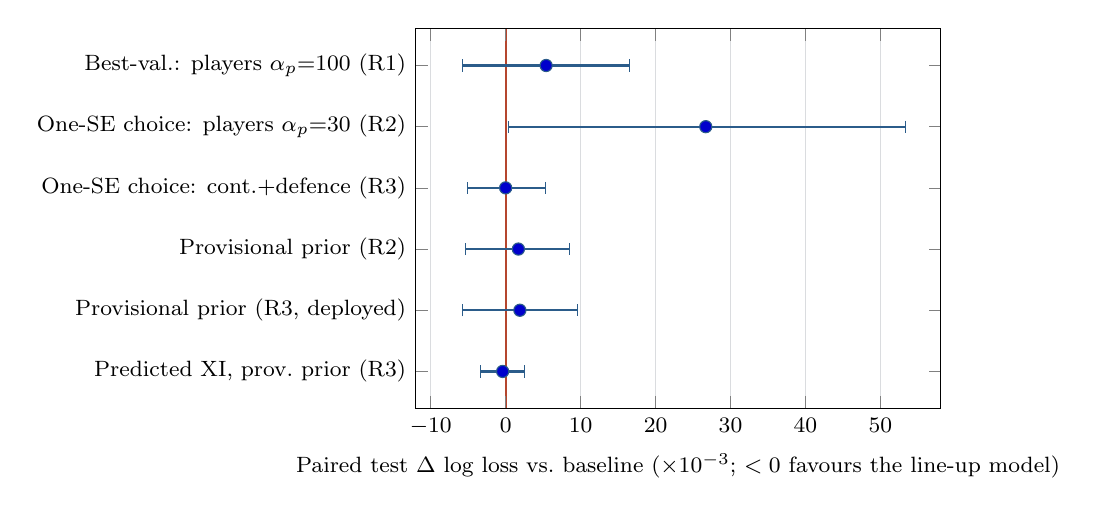
\begin{tikzpicture}
\begin{axis}[
  width=0.68\linewidth, height=6.4cm,
  xlabel={Paired test $\Delta$ log loss vs.\ baseline ($\times10^{-3}$; $<0$ favours the line-up model)},
  ytick={1,2,3,4,5,6},
  yticklabels={
    {Predicted XI, prov.\ prior (R3)},
    {Provisional prior (R3, deployed)},
    {Provisional prior (R2)},
    {One-SE choice: cont.+defence (R3)},
    {One-SE choice: players $\alpha_p{=}30$ (R2)},
    {Best-val.: players $\alpha_p{=}100$ (R1)}},
  yticklabel style={font=\footnotesize},
  xmin=-12, xmax=58, ymin=0.4, ymax=6.6,
  xmajorgrids, grid style={muted!25},
  tick label style={font=\footnotesize}, label style={font=\footnotesize},
  extra x ticks={0}, extra x tick style={grid style={warn,thick}},
  extra x tick labels={}]
\addplot+[only marks, mark=*, mark size=2.2pt, color=accent,
  error bars/.cd, x dir=both, x explicit, error bar style={thick}]
  coordinates {
    (-0.4,1) += (2.9,0) -= (2.9,0)
    (1.9,2)  += (7.7,0) -= (7.6,0)
    (1.7,3)  += (6.8,0) -= (7.1,0)
    (0.0,4)  += (5.3,0) -= (5.1,0)
    (26.7,5) += (26.6,0) -= (26.3,0)
    (5.4,6)  += (11.1,0) -= (11.1,0)
  };
\end{axis}
\end{tikzpicture}
\caption{Held-out test effect of each round's chosen model, with 95\% paired
bootstrap intervals over 160 test matches. Only one interval excludes zero, and
it lies on the \emph{wrong} side (round~2, player effects). R1--R3: evaluation
rounds (\cref{sec:rounds}).}
\label{fig:forest}
\end{figure}

\subsection{Posterior of the deployed layer}

\begin{table}[h]
\centering\small
\begin{tabular}{@{}llcc@{}}
\toprule
& Coefficient & Prior mean (sd) & Posterior mean $\pm$ sd\\
\midrule
$b_1$ & own discontinuity & $-0.15$ (0.15) & $-0.150\pm0.137$\\
$b_2$ & opponent discontinuity & $+0.10$ (0.15) & $-0.009\pm0.138$\\
$b_3$ & own absent goal share & $-0.25$ (0.15) & $-0.187\pm0.116$\\
$b_4$ & opponent absent goal share & $\phantom{+}0.00$ (0.10) & $-0.008\pm0.087$\\
$b_5$ & opponent defensive discontinuity & $+0.20$ (0.15) & $+0.046\pm0.126$\\
\bottomrule
\end{tabular}
\caption{Deployed coefficients (log-rate scale). Posterior sds are barely
smaller than prior sds, so the data are weakly informative. Where the data do
move the posterior ($b_2$, $b_5$), they move it \emph{towards zero}, against
the domain prior.}
\label{tab:posterior}
\end{table}

\subsection{Does line-up information help at all?}\label{sec:res-missing}

We hid a random share of players' line-up indicators on the test folds,
replacing them by typical start rates.

\begin{figure}[h]
\centering
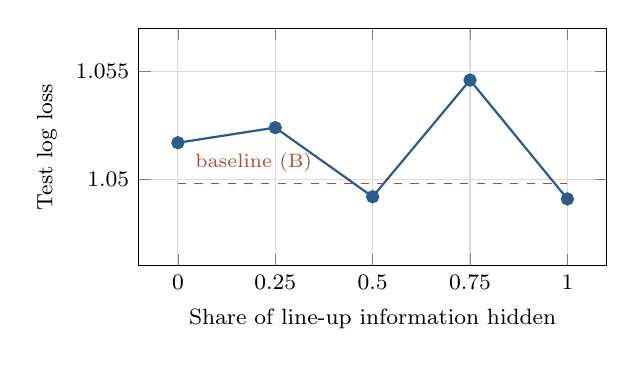
\begin{tikzpicture}
\begin{axis}[width=0.62\linewidth,height=4.6cm,
  xlabel={Share of line-up information hidden}, ylabel={Test log loss},
  xtick={0,0.25,0.5,0.75,1}, ymin=1.046, ymax=1.057,
  yticklabel style={/pgf/number format/fixed,/pgf/number format/precision=3},
  tick label style={font=\footnotesize}, label style={font=\footnotesize},
  grid=major, grid style={muted!25}]
\addplot[thick,mark=*,color=accent] coordinates
  {(0,1.0517) (0.25,1.0524) (0.5,1.0492) (0.75,1.0546) (1,1.0491)};
\addplot[dashed,color=warn,domain=0:1] {1.0498};
\node[font=\scriptsize,color=warn,anchor=south west] at (axis cs:0.02,1.0499) {baseline (B)};
\end{axis}
\end{tikzpicture}
\caption{No monotone trend. Removing all line-up information is as good as
keeping it, so in this sample line-up information has no measurable predictive
value at the match-outcome level.}
\label{fig:missing}
\end{figure}

\subsection{Calibration}

\begin{figure}[h]
\centering
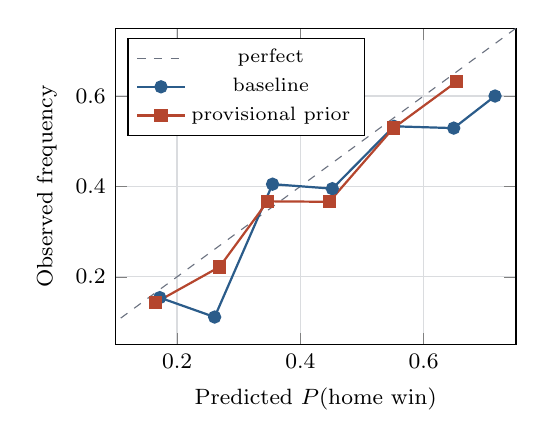
\begin{tikzpicture}
\begin{axis}[width=0.55\linewidth,height=5.6cm,
  xlabel={Predicted $P(\text{home win})$}, ylabel={Observed frequency},
  xmin=0.1,xmax=0.75,ymin=0.05,ymax=0.75,
  legend style={font=\scriptsize,at={(0.03,0.97)},anchor=north west},
  tick label style={font=\footnotesize}, label style={font=\footnotesize},
  grid=major, grid style={muted!25}]
\addplot[muted,dashed,domain=0:1] {x};
\addlegendentry{perfect}
\addplot[color=accent,mark=*,thick] coordinates
  {(0.172,0.154) (0.261,0.111) (0.355,0.405) (0.452,0.395) (0.552,0.533) (0.649,0.529) (0.716,0.600)};
\addlegendentry{baseline}
\addplot[color=warn,mark=square*,thick] coordinates
  {(0.165,0.143) (0.269,0.222) (0.347,0.367) (0.447,0.366) (0.551,0.529) (0.654,0.632)};
\addlegendentry{provisional prior}
\end{axis}
\end{tikzpicture}
\caption{Reliability of home-win probabilities on the 160 test matches (bins
with $n\ge5$; bin sizes 5--41). Both are roughly calibrated, with a slight
over-prediction of home wins above $0.6$ for the baseline. Bins are too small
for strong claims.}
\label{fig:calib}
\end{figure}

Top-1 accuracy on the test folds is $0.469$ (baseline) and $0.481$
(provisional prior). This difference is not meaningful on 160 matches. The
actual draw rate is $28.1\%$; neither model ever has draw as its arg-max.

\subsection{Evaluation history and disclosure}\label{sec:rounds}

\begin{table}[h]
\centering\small
\begin{tabularx}{\linewidth}{@{}c>{\raggedright\arraybackslash}p{5.6cm}>{\raggedright\arraybackslash}X@{}}
\toprule
Round & Change & Outcome on test \\
\midrule
R1 & Select minimum-validation candidate & Player effects ($\alpha_p{=}100$): $+0.0054$ $[-0.0057,+0.0165]$. Not an improvement. \\
R2 & \emph{After viewing R1 test}: one-SE rule, goal-share feature, provisional prior & One-SE choice (players, $\alpha_p{=}30$) $+0.0267$ $[+0.0004,+0.0533]$: significantly worse. Prior deployed: $+0.0017$ $[-0.0054,+0.0085]$. \\
R3 & \emph{After R2 and a user request about individual players}: defensive-discontinuity feature, 5-dim prior & One-SE choice (continuity+defence) $+0.0000$ $[-0.0051,+0.0053]$; deployed prior $+0.0019$ $[-0.0057,+0.0096]$. \\
\bottomrule
\end{tabularx}
\caption{Each round was designed after seeing the previous round's test
results. The test folds are therefore \textbf{not an untouched holdout} for the
deployed configuration \citep{cawley2010}. The neutral R3 result is a sanity
check, not a confirmatory estimate.}
\label{tab:rounds}
\end{table}

% ================================================================== 8
\section{Case study (demonstration data)}\label{sec:case}

The demo replays a recorded FPL snapshot (4 Nov 2026) for Nottingham Forest
v.\ Manchester City (kickoff Sun 8 Nov, 01:30 HKT), with \textbf{simulated}
news from fictional publishers on \code{.invalid} domains. The figures below
were regenerated with the round-3 artifacts for this report.

\begin{table}[h]
\centering\small
\begin{tabularx}{\linewidth}{@{}lX@{}}
\toprule
Demo clock (UTC) & System output \\
\midrule
Wed 4 Nov 12:00 & ``No confirmed fixture tonight (17:00--06:00 HKT)''; offers Forest v City on 8 Nov. No probability is invented. \\
Sat 7 Nov 08:00 & Haaland's corroborated availability $\pi=0.31$ (doubtful; wire ``doubt'' + tabloid ``out'' and its syndicated copy merged). City: \textbf{52\%} win / 24\% draw / 24\% loss; baseline alone 55\%. Top contribution: Haaland availability, $-0.10$ City xG. \\
Same, what-if & ``Without Haaland'' vs.\ ``with'': City win $-3.7$ points. Likeliest replacements: Bouaddi (+0.21 start prob.), Foden (+0.11), Cherki (+0.10). \\
Sat 7 Nov 16:45 & Simulated official XIs ($T-60$\,min) replace predictions; Haaland starts ($\pi=0.98$). City \textbf{56\%}. Haaland's modelled absence cost: $-5.4$ win points, $-0.23$ xG. \\
\bottomrule
\end{tabularx}
\caption{Demo replay. All news is simulated; the numbers illustrate mechanics, not accuracy.}
\label{tab:case}
\end{table}

The replay also exposes model artefacts, discussed in \cref{sec:flaws}. City's
goalkeeper's absence lowers \emph{City's own} xG ($-0.10$) far more than it
raises Forest's ($+0.01$). A Forest defender carries a $29\%$ share of Forest's
recent goals and so ranks as Forest's most valuable starter.

% ================================================================== 9
\section{Software validation}\label{sec:tests}

The repository's test suite (88 tests, all passing in about two minutes,
offline) includes targeted MatchSense tests for alias resolution and timezone
windows, ``tonight'' with no fixture, conflicting and syndicated reports,
precedence of confirmed statements, the no-probability LLM contract,
eleven-player XI validity, official-XI override, ambiguous player names,
probabilities summing to one, missing credentials, cache retry and stale
fallback, in-progress and unsupported competitions, and the four leakage tests
of \cref{sec:design}. The tests check engineering invariants. They cannot check
forecasting skill.

% ================================================================== 10
\section{Critical appraisal}\label{sec:appraisal}

\subsection{Strengths}\label{sec:pros}
\begin{enumerate}[label=\textbf{S\arabic*.}]
  \item \textbf{No LLM-generated probabilities.} The LLM's outputs are typed,
        validated and cached, and every LLM stage has a deterministic fallback.
        This removes the most common failure of ``AI predictor'' products.
  \item \textbf{Honest reporting.} The baseline is always displayed. The
        line-up layer is labelled provisional in every response. Negative
        results and post-hoc changes are documented in the repository.
  \item \textbf{Leakage discipline.} Strict time cut-offs, snapshotting and
        mutation tests at four points, plus fold audits in the artifacts.
  \item \textbf{A validated baseline.} The Poisson model beats a
        class-frequency prior by $0.054$ log loss on an untouched season and is
        not improved by a logistic alternative.
  \item \textbf{A useful selection model.} Start probabilities improve log
        loss by 13\% relative over a heuristic.
  \item \textbf{Evidence provenance.} Every belief links to sourced,
        timestamped, de-duplicated items. Conflicts are surfaced, not averaged
        away silently.
  \item \textbf{Safe refusals.} The system answers ``no fixture'', ``match in
        progress'' and ``competition not modelled'' rather than inventing
        numbers. It degrades gracefully without API keys.
  \item \textbf{Coherent uncertainty.} The Monte Carlo propagates both line-up
        and coefficient uncertainty, and probabilities sum to one by
        construction.
\end{enumerate}

\subsection{Flaws and weaknesses}\label{sec:flaws}

\Cref{tab:flaws} lists concrete flaws, each with a severity for the system's
stated purpose of answering ``will X win?'' with news awareness.

\begin{table}[p]
\centering\small
\renewcommand{\arraystretch}{1.15}
\begin{tabularx}{\linewidth}{@{}>{\raggedright\arraybackslash}p{3.6cm}X>{\centering\arraybackslash}p{1.4cm}@{}}
\toprule
Flaw & Evidence and consequence & Severity\\
\midrule
F1.~News channel has no demonstrated value & Line-up effects are not identified (\cref{fig:forest,fig:missing}), and news enters \emph{only} through line-ups. The headline feature, ``news-aware'', moves probabilities by priors, not by measured effects. & \sev{High}\\
F2.~Contaminated test folds & Three rounds were designed after viewing test results (\cref{tab:rounds}). No clean estimate of the deployed model's skill exists. & \sev{High}\\
F3.~One season of line-up data & 700 team-match observations against football's high outcome variance. Player effects are unidentifiable \citep{kharrat2020}. & \sev{High}\\
F4.~Hand-set evidence constants & The availability table, certainty weights, credibilities and 36\,h half-life are editorial. Some cells are counter-intuitive (``doubtful+speculation'' $\to0.6$ is \emph{more} available than ``doubtful+confirmed'' $\to0.5$). None is calibrated. & Medium\\
F5.~Mis-attributed positional effects & The goalkeeper's absence mostly lowers his own team's attack (\cref{sec:case}). Team-level features cannot distinguish roles, and $b_5$ was pulled towards zero. & Medium\\
F6.~Noisy goal shares & Short decayed windows give defenders 29\% goal shares; set pieces and own goals are mixed with open play. The ``most valuable player'' ranking is unstable. & Medium\\
F7.~Draws never predicted & Draw recall is 0 in every model (28\% of matches). Probabilities are fine, but the top-1 headline can never say ``draw''. & Medium\\
F8.~Weak on upsets & Upset log loss $1.29$ vs.\ $1.06$ for the prior: the model is over-confident in favourites when they lose. & Medium\\
F9.~Train/serve source shift & The selection model is trained on openfootball line-ups, but live features come from FPL histories (differing minute and position conventions). This is untested. & Medium\\
F10.~Associational ``what-if'' & Counterfactuals use coefficients confounded by rotation against weak opponents and fixture congestion. They are not causal effects \citep{hernan2020}. & Medium\\
F11.~Coarse positions & FPL classes (wingers are ``MID'') make formations and the defensive unit approximate. The code enforces ``back line $\ge$ usual size'', whereas the model doc says ``$\ge3$''. & Low\\
F12.~Approximate XI sampler & Greedy Gumbel top-$k$ under caps is not exact conditional-Bernoulli sampling \citep{chen1994}, so marginals do not exactly equal $p_i\pi_i$. & Low\\
F13.~Fragile data supply & FPL endpoints are undocumented, free NewsAPI is delayed, and cup fixtures need a key; otherwise answers must caveat that cup matches cannot be ruled out. & Low\\
F14.~Query cost and latency & A new question through Codex costs about 20k tokens and 15\,s (repeats are cached). This is heavy for parsing a short sentence. & Low\\
F15.~Static baseline & The \code{ScoreModel} is not refitted in-season; only its state rolls forward. Drift within 2026-27 is uncorrected. & Low\\
F16.~Scope & Premier League only, pre-match only, no player transfer of effects across clubs, tactical news not quantified. & Low\\
\bottomrule
\end{tabularx}
\caption{Flaws identified from the evaluation artifacts, a code review and a
replay of the demo.}
\label{tab:flaws}
\end{table}

\subsection{Pros and cons versus simpler alternatives}

\begin{table}[h]
\centering\small
\begin{tabularx}{\linewidth}{@{}l>{\raggedright\arraybackslash}X>{\raggedright\arraybackslash}X@{}}
\toprule
Alternative & Pros relative to MatchSense & Cons relative to MatchSense\\
\midrule
Baseline \code{ScoreModel} alone & Same measured accuracy; simpler; no news pipeline or keys; nothing provisional. & Cannot answer ``what if X is out?''; ignores confirmed line-ups; no evidence trail. \\
Ask an LLM directly & Trivial to build; fluent; reads any source. & Uncalibrated, unverifiable numbers; hallucinated fixtures and injuries \citep{ji2023}; no backtest possible. \\
Bookmaker / betting-market odds & Aggregate private information; typically sharper than public models \citep{dixon1997}. & Include a margin; no explanation; no what-if; access and terms restrictions. \\
Event-data player models (VAEP, xG) & Can identify player value with far more data \citep{decroos2019}. & Need licensed event data; heavy engineering; still confounded for selection. \\
\bottomrule
\end{tabularx}
\caption{Positioning. For pure accuracy, MatchSense currently equals its own
baseline. Its distinct value lies in transparency, refusal behaviour,
evidence tracing and scenario analysis.}
\label{tab:proscons}
\end{table}

\subsection{Threats to validity}
\begin{description}[style=unboxed,leftmargin=0pt]
  \item[Internal.] One season; post-hoc design changes (F2); availability
        constants are assumptions (F4); test-fold bins are small.
  \item[Construct.] Discontinuity and goal share are crude proxies for player
        quality; defensive value is barely represented; positions are coarse.
  \item[External.] One league with a stable top tier. The model refuses other
        competitions, but within-league regime changes (new managers, promoted
        sides) are only partly captured by the baseline's state transitions.
  \item[Conclusion.] With 160 test matches, a paired log-loss interval has a
        half-width of about $0.005$--$0.01$. Effects smaller than this, which
        is plausibly where real line-up effects lie, are undetectable.
\end{description}

\subsection{Responsible use}
Football forecasts are commonly used for betting. MatchSense's probabilities
are roughly calibrated but carry no demonstrated edge, and the news layer is
explicitly unvalidated. The system should not be used as a basis for wagering.
The demo's news is simulated and must never be cited as fact. Only headline,
summary, link and time are used from RSS feeds, and pages that forbid scraping
are not fetched.

% ================================================================== 11
\section{Future work}\label{sec:future}
\begin{enumerate}
  \item \textbf{More line-up seasons} with hierarchical shrinkage of player
        effects \citep{baio2010,kharrat2020}, ideally with event-level xG.
  \item \textbf{Prospective news archiving.} Store every retrieved item with
        its timestamp so that the news channel itself can be evaluated
        without leakage in a future season.
  \item \textbf{Calibrate the evidence constants} (F4) against FPL's own
        chance-of-playing outcomes, which are observable after each match.
  \item \textbf{Role-aware impact features} (keeper, centre-back, striker) to
        fix F5, and an explicit draw-decision rule for the top-1 headline (F7).
  \item \textbf{A pre-registered, untouched evaluation} on 2026-27 with the
        configuration frozen now, using the prediction store's pre-kickoff
        scoring.
  \item \textbf{Cheaper query parsing}: a small local model or the rule parser
        first, with the LLM only when the rules fail.
\end{enumerate}

% ================================================================== 12
\section{Conclusion}\label{sec:conclusion}
MatchSense shows how to connect unstructured football news to a validated
forecaster without letting a language model invent probabilities. Evidence is
typed, sourced, time-stamped and corroborated, and it enters the model only
through player availability and line-up simulation. The evaluation separates
what works from what does not. The goal-based baseline and the start-probability
model are validated out of sample. Line-up effects on goal rates are not
identified from one season, and the most expressive specification overfits.
The deployed news adjustment is a labelled, prior-dominated model whose
held-out effect is indistinguishable from zero. The system's present value is
transparency, safe refusal and scenario analysis, not accuracy beyond its
baseline. Whether news adds accuracy remains an open question. The project's
own infrastructure (timestamped evidence and pre-kickoff prediction scoring) is
what can answer it on a future season.

% ------------------------------------------------------------------ refs
\bibliographystyle{plainnat}
\bibliography{references}

% ------------------------------------------------------------------ appendix
\appendix
\section{Reproducibility}\label{app:repro}
{\footnotesize
\begin{verbatim}
python -m src.scripts.train_season_simulator --source local   # baseline
python -m src.scripts.compare_match_outcomes ./england        # Table 2
python -m src.scripts.train_lineup_impact                     # Tables 3-6, Figs 2-4
python -m src.scripts.serve --demo                            # Section 8
python -m pytest                                              # Section 9
\end{verbatim}}
\noindent All commands are run with the project virtual environment
(\code{./.venv/bin/python}).
Artifacts: \code{artifacts/walk\_forward\_comparison/REPORT.md};
\code{artifacts/matchsense/\{metrics.json, REPORT.md, REPORT\_round1.md,
REPORT\_round2.md\}}. Software: Python 3.15.0, scikit-learn 1.9.1, SciPy
1.18.1, NumPy 2.5.4, FastAPI 0.162. Seeds: bootstrap 7; missing-data masks 11;
Monte Carlo 20261104.

\section{Data availability}
openfootball/england is public domain. The FPL endpoints are public but
undocumented. BBC Sport RSS is used for headline, summary, link and time only.
The demonstration news and official line-ups are simulated.

\end{document}
